\documentclass[10pt,letterpaper]{amspset}
\usepackage{fullpage}
\usepackage{gensymb}
\usepackage{graphicx}
\usepackage{tikz}
\usepackage{amsmath}
\usepackage{pgfplots}
\pgfplotsset{compat=1.17}
\graphicspath{ {./images/} }
\notag

% info for header block in upper right hand corner
\name{Brady Lamson}
\class{MATH 1120 SPRING 2021}
\assignment{Graphing Trig Functions Part 1}
\duedate{Feb 16th}

\begin{document}

\problemlist{Graphs of the Trigonometric Functions Part I:  

10.5: 1-9, 13-22, 25, 26}

For exercises 1--9, graph one cycle of the given function. State the period, amplitude, phase shift and vertical shift of the function.

\begin{problem}[1]
    $y = 3 sin(x)$
\end{problem}

\begin{solution} 
    Before we begin let's first describe what we'll be working with. 
    \[ f(x) = a \cdot \sin(bx + c) + d \]
   
   \begin{center}
        a = amplitude \\
        b = period (default being $2\pi$)\\
        c = phase shift \\
        d = vertical shift \\
   \end{center} 
   
   From here we can start to examine exactly what is going on.  What we can see is that only the $a$ is here to transform our sine function. So, this guy affects the amplitude. It's a simple vertical stretch by 3, meaning our new maximum and minimum is 3 and -3 respectively. 
   
   As that is all that is changed the period, phase shift and vertical shift are all unaffected. 
   \medskip
   
   \noindent $y = 3 sin(x)$ \\
    Period : $2\pi$ \\
    Amplitude : 3 \\
    Phase Shift : 0 \\
    Vertical Shift : 0 \\
   
   
    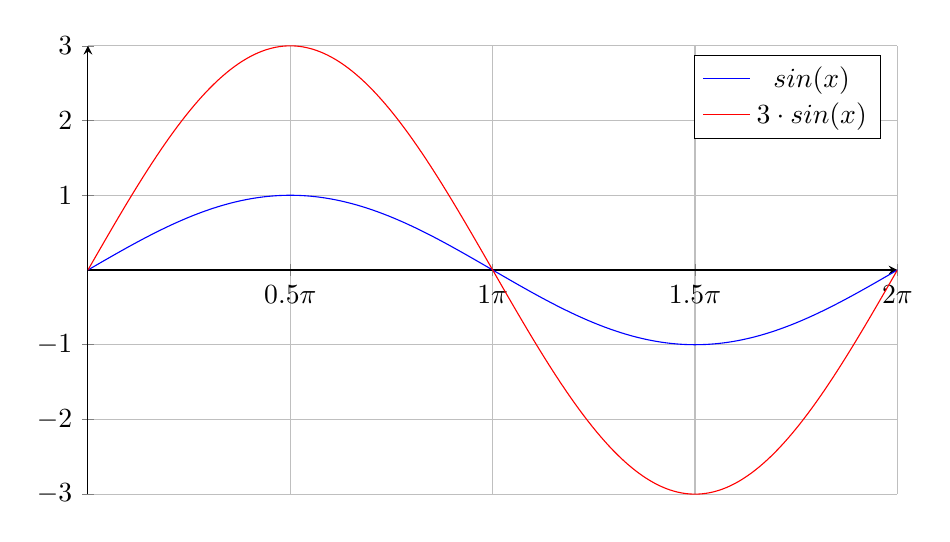
\begin{tikzpicture}
        \begin{axis}
            [
            grid=both,
            axis lines=middle,
            domain=0:2*pi,
            samples=200,
            no marks,
            xticklabels={-2$\pi$,-1.5$\pi$,...$\pi$,2$\pi$},
            xtick={-6.2832,-4.7124,...,6.2832},
            x post scale=1.5
            ]
            \addplot {sin(deg(x))};
            \addlegendentry{$sin(x)$};
            \addplot {3 * sin(deg(x))};
            \addlegendentry{$3 \cdot sin(x)$};
        \end{axis}
    \end{tikzpicture}
\end{solution}


\pagebreak


\begin{problem}[2]
    $y = sin(3x)$
\end{problem}

\begin{solution}[Solution]
    The three before the x here indicates that we will have a change in period. What we can do to solve for the new period is set $3x = 2\pi$ and solve. What we should see is a smaller period, which implies that the graph will be completing cycles "faster" than the default sine graph. 
    
    \[ 3x = 2\pi \]
    \[\boxed{ x = \frac{2\pi}{3} }\]
    
    We can safely say that everything else is unaffected so amplitude, phase shift and vertical shift are all the same as normal.
    \medskip 
    
    
    \noindent $y = 3 sin(x)$ \\[+2mm]
    Period : $\frac{2\pi}{3}$ \\[+2mm]
    Amplitude : 1 \\[+2mm]
    Phase Shift : 0 \\[+2mm]
    Vertical Shift : 0 \\
   
   
   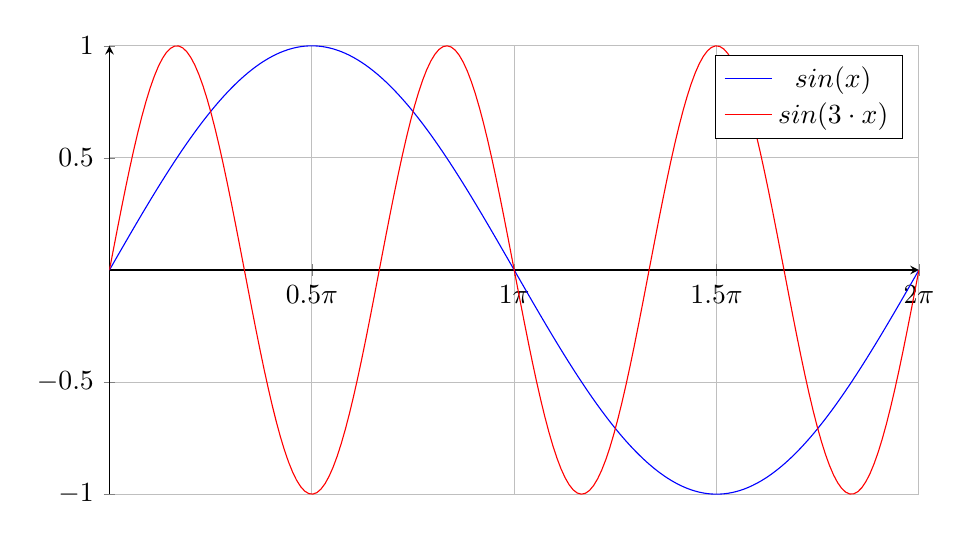
\begin{tikzpicture}
        \begin{axis}
            [
            grid=both,
            axis lines=middle,
            domain=0:2*pi,
            samples=200,
            no marks,
            xticklabels={-2$\pi$,-1.5$\pi$,...$\pi$,2$\pi$},
            xtick={-6.2832,-4.7124,...,6.2832},
            x post scale=1.5
            ]
            \addplot {sin(deg(x))};
            \addlegendentry{$sin(x)$};
            \addplot {sin(deg(3 * x))};
            \addlegendentry{$sin(3 \cdot x)$};
        \end{axis}
    \end{tikzpicture}
\end{solution}


\pagebreak


\begin{problem}[3]
    $y = -2 \cdot cos(x)$
\end{problem}

\begin{solution}[Solution]
    As we know from problem one the \textbf{-2} in the \textbf{a} spot will be affecting our amplitude. The negative value indicates that our function will be flipped and stretched by 2. This makes sense when you think about a negative angle $\theta$. With $-\theta$ we would be going around the circle backwards. So when cosine would be negative and positive will be flipped. Anyway, from this alone we can say that the \textbf{amplitude will be -2} and the \textbf{rest will be the same}.
    \medskip
   
    \noindent $y = -2 \cdot cos(x)$ \\[+2mm]
    Period : $2\pi$ \\[+2mm]
    Amplitude : -2 \\[+2mm]
    Phase Shift : 0 \\[+2mm]
    Vertical Shift : 0 \\
   
   
   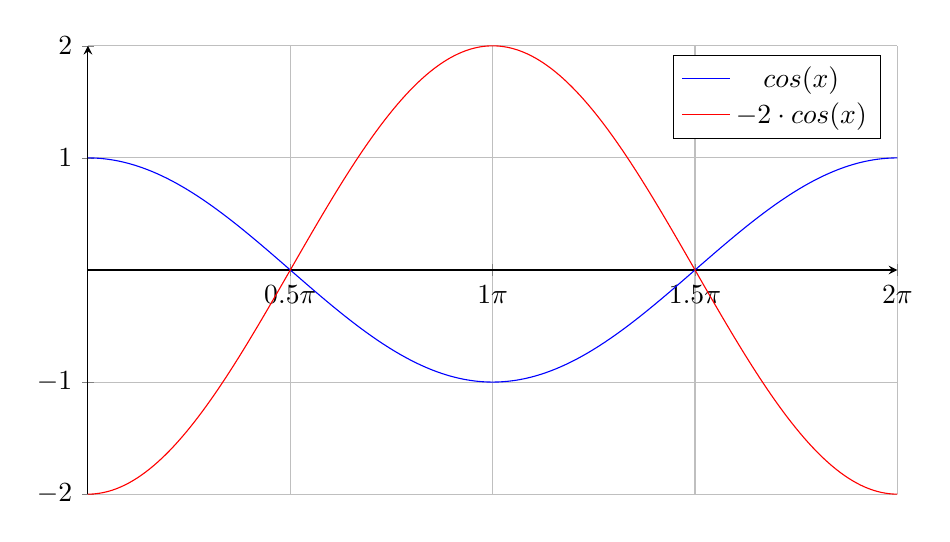
\begin{tikzpicture}
        \begin{axis}
            [
            grid=both,
            axis lines=middle,
            domain=0:2*pi,
            samples=200,
            no marks,
            xticklabels={-2$\pi$,-1.5$\pi$,...$\pi$,2$\pi$},
            xtick={-6.2832,-4.7124,...,6.2832},
            x post scale=1.5
            ]
            \addplot {cos(deg(x))};
            \addlegendentry{$cos(x)$};
            \addplot {-2 * cos(deg(x))};
            \addlegendentry{$-2 \cdot cos(x)$};
        \end{axis}
    \end{tikzpicture}
\end{solution}


\pagebreak


\begin{problem}[4]
    $y = cos(x - \frac{\pi}{2})$
\end{problem}

\begin{solution}[Solution]
    So we have our first phase shift here. All this means is that the graph will be identical to the normal cosine graph aside from one difference. That difference is that it will be shifted to the right by $\frac{\pi}{2}$. Why to the right? If we remember from algebra, the horizontal shifts are flipped from where you would think they would go. Negative values indicate a shift to the right and positive values indicate a shift to the left. 
    \medskip
   
    \noindent $y = cos(x - \frac{\pi}{2})$ \\[+2mm]
    Period : $2\pi$ \\[+2mm]
    Amplitude : 1 \\[+2mm]
    Phase Shift : $\frac{\pi}{2}$ \\[+2mm]
    Vertical Shift : 0 \\
   
   
   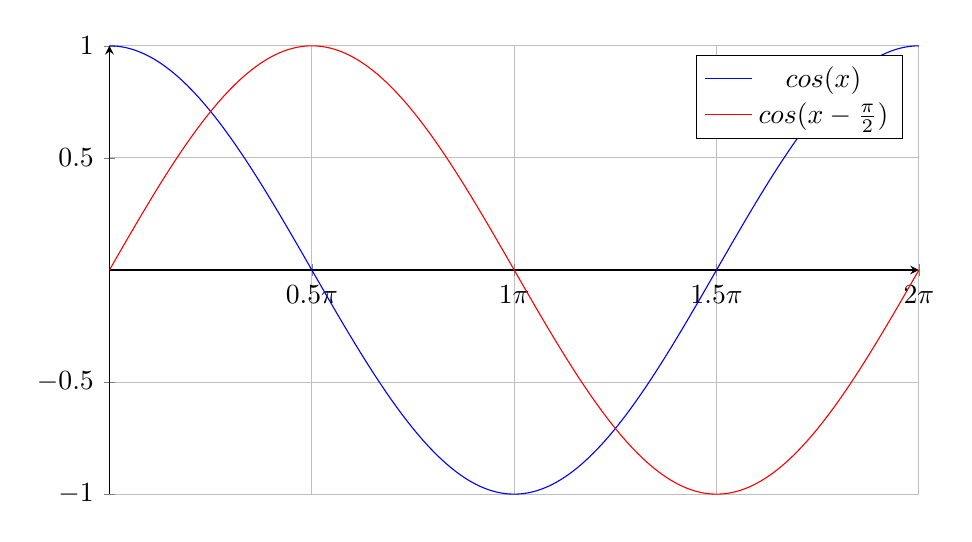
\begin{tikzpicture}
        \begin{axis}
            [
            grid=both,
            axis lines=middle,
            domain=0:2*pi,
            samples=200,
            no marks,
            xticklabels={-2$\pi$,-1.5$\pi$,...$\pi$,2$\pi$},
            xtick={-6.2832,-4.7124,...,6.2832},
            x post scale=1.5
            ]
            \addplot {cos(deg(x))};
            \addlegendentry{$cos(x)$};
            \addplot {cos(deg(x - (pi / 2))};
            \addlegendentry{$cos(x - \frac{\pi}{2})$};
        \end{axis}
    \end{tikzpicture}
\end{solution}


\pagebreak


\begin{problem}[5]
    $y = -sin(x + \frac{\pi}{3})$
\end{problem}

\begin{solution}[Solution]
    Now things get slightly more interesting. This will be both a \textbf{flip} due to the negative sine and a \textbf{shift to the left by $\frac{\pi}{3}$.} \textbf{Period, amplitude and vertical shift will all be their default values here.}
    \medskip 
    

    \noindent $y = -sin(x + \frac{\pi}{3})$ \\[+2mm]
    Period : $2\pi$ \\[+2mm]
    Amplitude : 1 \\[+2mm]
    Phase Shift : $-\frac{\pi}{3}$ \\[+2mm]
    Vertical Shift : 0 \\

   
   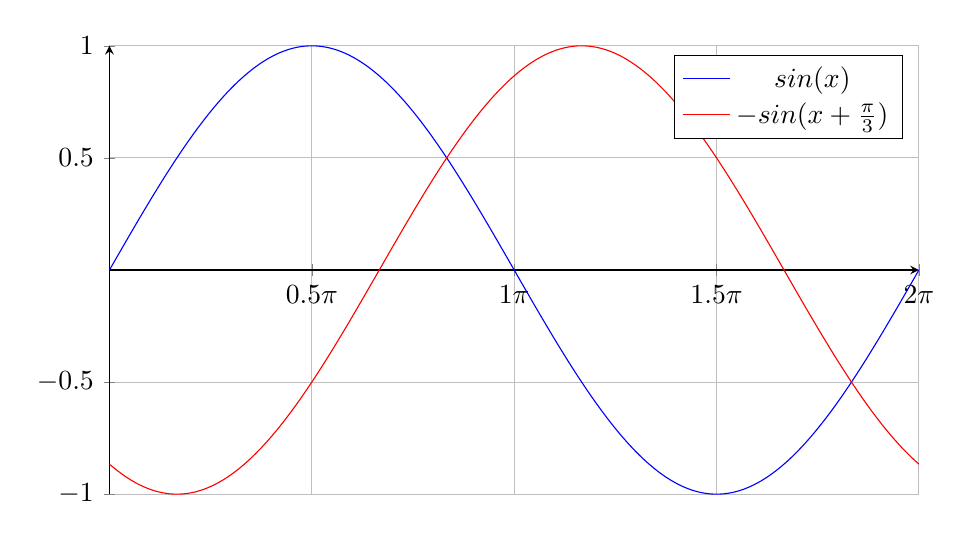
\begin{tikzpicture}
        \begin{axis}
            [
            grid=both,
            axis lines=middle,
            domain=0:2*pi,
            samples=200,
            no marks,
            xticklabels={-2$\pi$,-1.5$\pi$,...$\pi$,2$\pi$},
            xtick={-6.2832,-4.7124,...,6.2832},
            x post scale=1.5
            ]
            \addplot {sin(deg(x))};
            \addlegendentry{$sin(x)$};
            \addplot {-sin(deg(x + (pi / 3))};
            \addlegendentry{$-sin(x + \frac{\pi}{3})$};
        \end{axis}
    \end{tikzpicture}
\end{solution}


\pagebreak


\begin{problem}[6]
    $y = sin(2x - \pi)$
\end{problem}

\begin{solution}[Solution]
    You know the drill by now. We need to solve for our new period first.
    
    \[ 2x = 2\pi \]
    \[\boxed{ x = \pi }\]
    
    From here it's simple, the graph will also be shifted to the right by $\pi$. Easy stuff. Actually, that's not true! shifts in trig graphs like these need an extra step when we have more going on. To solve for our phase shift we will use the formula $bx - c = 0$. Our $b$ is 2 and our $c$ is $\pi$.
    \[ 2x - \pi = 0 \]
    \[ 2x = \pi \]
    \[\boxed{ x = \frac{\pi}{2} }\]
    
    
    \noindent $y = sin(2x - \pi)$ \\[+2mm]
    Period : $\pi$ \\[+2mm]
    Amplitude : 1 \\[+2mm]
    Phase Shift : $\frac{\pi}{2}$ \\[+2mm]
    Vertical Shift : 0 \\
   
   
   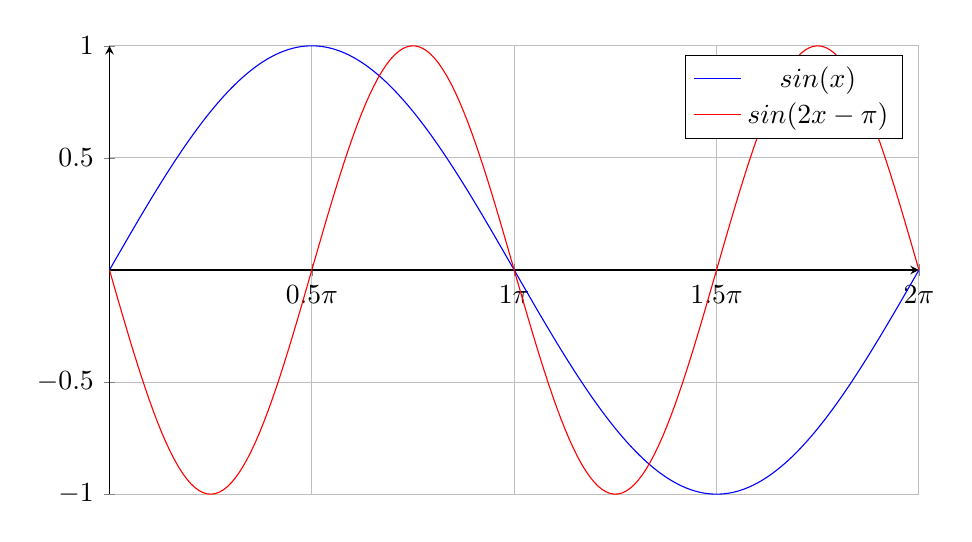
\begin{tikzpicture}
        \begin{axis}
            [
            grid=both,
            axis lines=middle,
            domain=0:2*pi,
            samples=200,
            no marks,
            xticklabels={-2$\pi$,-1.5$\pi$,...$\pi$,2$\pi$},
            xtick={-6.2832,-4.7124,...,6.2832},
            x post scale=1.5
            ]
            \addplot {sin(deg(x))};
            \addlegendentry{$sin(x)$};
            \addplot {sin(deg((2 * x) - pi))};
            \addlegendentry{$sin(2x - \pi{})$};
        \end{axis}
    \end{tikzpicture}
\end{solution}


\pagebreak


\begin{problem}[7]
    $y = -\frac{1}{3} cos (\frac{1}{2}x + \frac{\pi}{3})$
\end{problem}

\begin{solution}[Solution]
    Now we get to combine everything aside from the vertical shift together! First, the period.
    
    \[ \frac{1}{2}x = 2\pi \]
    \[\boxed{ x = 4\pi }\]
    
    Next, let's look at our amplitude. Amplitude is just the absolute value of a. Our a in this case being $-\frac{1}{3}$. The absolute value of which being $\frac{1}{3}$.
    
    After that we need to check out our phase shift using the same formula as last time!
    \[ bx - c = 0 \]
    \[ \frac{1}{2}x - \frac{\pi}{3} = 0 \]
    \[ \frac{1}{2}x = \frac{\pi}{3} \]
    \[ x = \frac{\pi}{3} \cdot \frac{2}{1} \]
    \[\boxed{ x = \frac{2\pi}{3} }\]
    
    
    \noindent $y = -\frac{1}{3} cos (\frac{1}{2}x + \frac{\pi}{3})$ \\[+2mm]
    Period : $4\pi$ \\[+2mm]
    Amplitude : $\frac{1}{3}$ \\[+2mm]
    Phase Shift : $\frac{2\pi}{3}$ \\[+2mm]
    Vertical Shift : 0 \\
   
   
   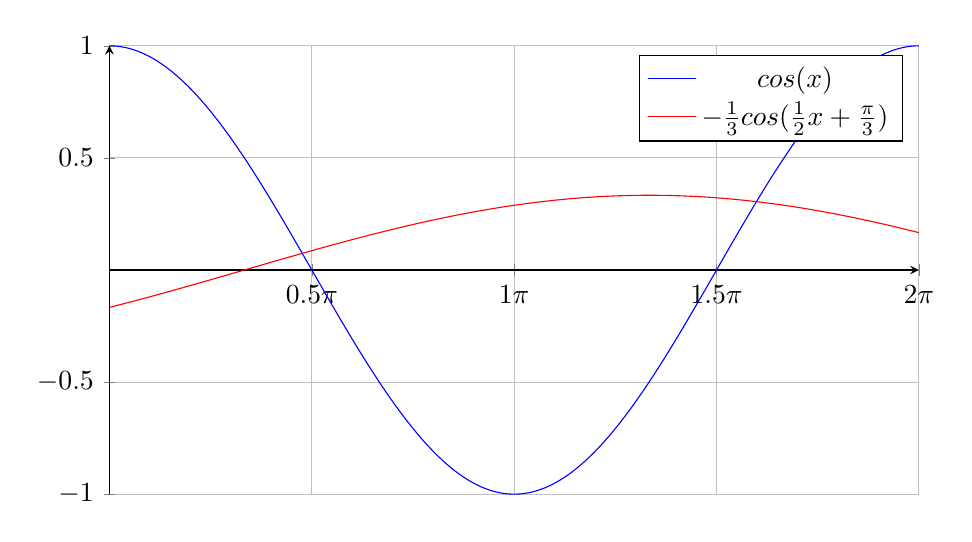
\begin{tikzpicture}
        \begin{axis}
            [
            grid=both,
            axis lines=middle,
            domain=0:2*pi,
            samples=200,
            no marks,
            xticklabels={-2$\pi$,-1.5$\pi$,...$\pi$,2$\pi$},
            xtick={-6.2832,-4.7124,...,6.2832},
            x post scale=1.5
            ]
            \addplot {cos(deg(x))};
            \addlegendentry{$cos(x)$};
            \addplot {(-1/3) * cos(deg((.5 * x) + (pi/3))};
            \addlegendentry{$-\frac{1}{3} cos (\frac{1}{2}x + \frac{\pi}{3})$};
        \end{axis}
    \end{tikzpicture}
\end{solution}


\pagebreak


\begin{problem}[8]
    $y = cos (3x - 2\pi) + 4$
\end{problem}

\begin{solution}[Solution]
    The only new thing here is the vertical shift at the end, and we'll get there. For now we'll use the same logic as the previous problems. First we solve for the period.
    
    \[ 3x = 2\pi \]
    \[\boxed{ x = \frac{2\pi}{3} }\]
    
    After that we need to check out our phase shift using the same formula as last time!
    \[ bx - c = 0 \]
    \[ 3x - 2\pi = 0 \]
    \[ 3x = 2\pi \]
    \[\boxed{ x = \frac{2\pi}{3} }\]
    
    Vertical shift is easy, it's just d which in this case is positive 4. If you're wondering about the amplitude, it will be the same. 
    
    \noindent $y = cos (3x - 2\pi) + 4$ \\[+2mm]
    Period : $\frac{2\pi}{3}$ \\[+2mm]
    Amplitude : $1$ \\[+2mm]
    Phase Shift : $\frac{2\pi}{3}$ \\[+2mm]
    Vertical Shift : 4 \\
   
   
   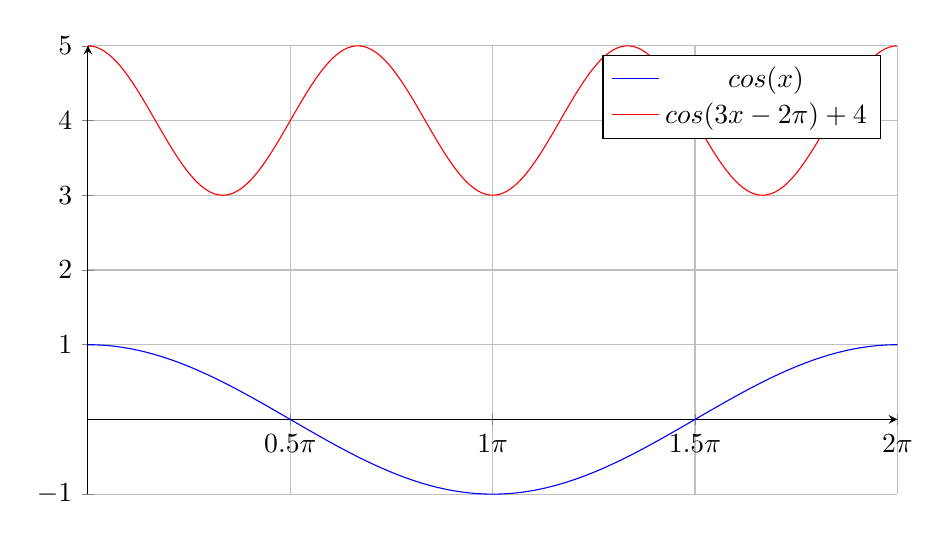
\begin{tikzpicture}
        \begin{axis}
            [
            grid=both,
            axis lines=middle,
            domain=0:2*pi,
            samples=200,
            no marks,
            xticklabels={-2$\pi$,-1.5$\pi$,...$\pi$,2$\pi$},
            xtick={-6.2832,-4.7124,...,6.2832},
            x post scale=1.5
            ]
            \addplot {cos(deg(x))};
            \addlegendentry{$cos(x)$};
            \addplot {(cos(deg((3*x) - (2 * pi)))+ 4)};
            \addlegendentry{$cos(3x - 2\pi) + 4$};
        \end{axis}
    \end{tikzpicture}
\end{solution}


\pagebreak


\begin{problem}[9]
    $y = sin (-x - \frac{\pi}{4}) - 2$
\end{problem}

\begin{solution}[Solution]
    The period will be the same. Even though it's negative sine is symmetrical along the y axis so this doesn't actually change anything. So the period will be $2\pi$. 
    
    After that we need to check out our phase shift. For this we can actually break out an identity. We know that $sin(-\theta) = -sin(\theta)$. We can use this to help us out. 
    \[ bx - c = 0 \]
    \[ x - \frac{\pi}{4} = 0 \]
    \[\boxed{ x = \frac{\pi}{4} }\]
    
    Vertical shift will be -2. This means the graph will be shifted down by 2. 
    
    \noindent $y = sin (-x - \frac{\pi}{4}) - 2$ \\[+2mm]
    Period : $2\pi$ \\[+2mm]
    Amplitude : $1$ \\[+2mm]
    Phase Shift : $-\frac{\pi}{4}$ \\[+2mm]
    Vertical Shift : -2 \\
   
   
   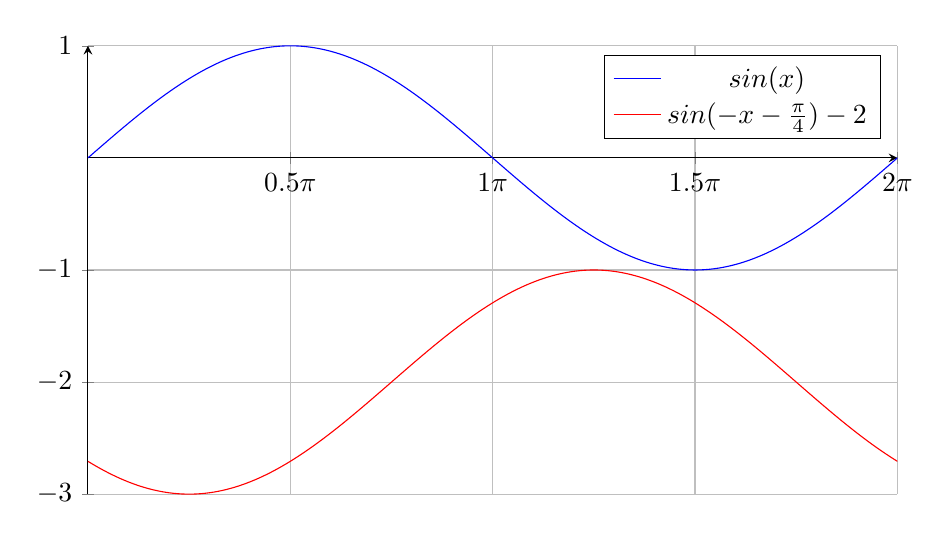
\begin{tikzpicture}
        \begin{axis}
            [
            grid=both,
            axis lines=middle,
            domain=0:2*pi,
            samples=200,
            no marks,
            xticklabels={-2$\pi$,-1.5$\pi$,...$\pi$,2$\pi$},
            xtick={-6.2832,-4.7124,...,6.2832},
            x post scale=1.5
            ]
            \addplot {sin(deg(x))};
            \addlegendentry{$sin(x)$};
            \addplot {(sin(deg((-x) - (pi / 4))) - 2)};
            \addlegendentry{$sin (-x - \frac{\pi}{4}) - 2$};
        \end{axis}
    \end{tikzpicture}
\end{solution}


\pagebreak


For exercises 13--22, graph one cycle of the given function. State the period of the function.

\begin{problem}[13]
    $y = tan (x - \frac{\pi}{3})$
\end{problem}

\begin{solution}[Solution]
    
    So, it is important to note that the default period of the tangent is $1\pi$. As this problem does not have anything that would change the period, that is still the case for this function. 
    
      \begin{tikzpicture}
        \begin{axis}
            [
            grid=both,
            axis lines=middle,
            domain= -1.5*pi:1.5*pi,
            ymin=-10,ymax=10,
            samples=200,
            no marks,
            xticklabels={-2$\pi$,-1.5$\pi$,...$\pi$,2$\pi$},
            xtick={-6.2832,-4.7124,...,6.2832},
            x post scale=1.5
            ]
            \addplot {tan(deg(x))};
            \addlegendentry{$tan(x)$};
            \addplot {(tan(deg(x - (pi / 3))))};
            \addlegendentry{$tan(x - \frac{\pi}{3})$};
        \end{axis}
    \end{tikzpicture}
\end{solution}


\begin{problem}[16]
    $y = sec (x - \frac{\pi}{2})$
\end{problem}

\begin{solution}[Solution]
    
    So, it is important to note that the default period of secant is the same as cosine, $2\pi$. As this problem does not have anything that would change the period, that is still the case for this function. 
    
      \begin{tikzpicture}
        \begin{axis}
            [
            grid=both,
            axis lines=middle,
            restrict x to domain*= -1.5*pi:1.5*pi,
            ymin=-10,ymax=10,
            samples=200,
            no marks,
            xticklabels={-2$\pi$,-1.5$\pi$,...$\pi$,2$\pi$},
            xtick={-6.2832,-4.7124,...,6.2832},
            x post scale=1.5
            ]
            \addplot {sec(deg(x))};
            \addlegendentry{$sec(x)$};
            \addplot {(sec(deg(x - (pi / 2))))};
            \addlegendentry{$sec(x - \frac{\pi}{2})$};
        \end{axis}
    \end{tikzpicture}
\end{solution}


\pagebreak


\begin{problem}[17]
    $y = - csc (x + \frac{\pi}{2})$
\end{problem}

\begin{solution}[Solution]
    
    So, it is important to note that the default period of cosecant is the same as sine, $2\pi$. As this problem does not have anything that would change the period, that is still the case for this function. 
    
      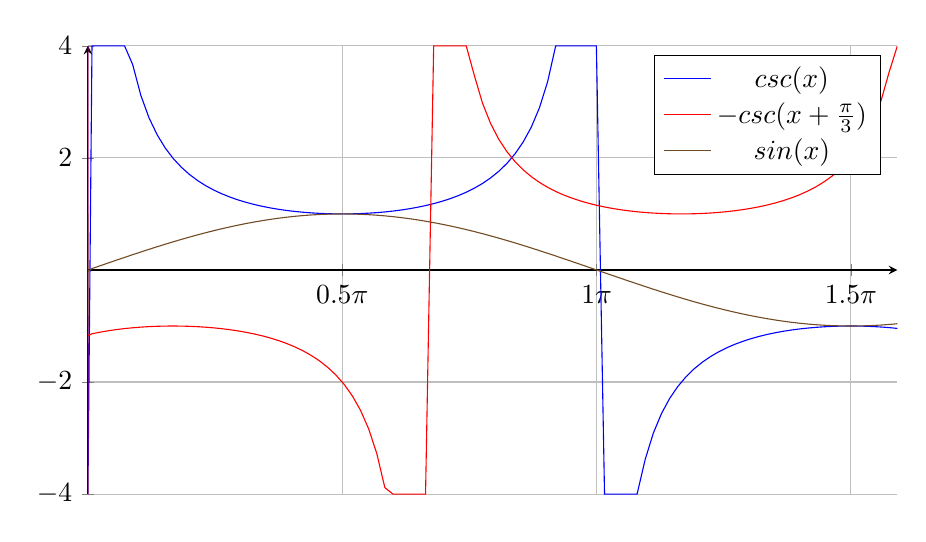
\begin{tikzpicture}
        \begin{axis}
            [
            grid=both,
            axis lines=middle,
            restrict x to domain*= 0:2*pi,
            restrict y to domain*= -4:4,
            samples=200,
            no marks,
            xticklabels={-2$\pi$,-1.5$\pi$,...$\pi$,2$\pi$},
            xtick={-6.2832,-4.7124,...,6.2832},
            x post scale=1.5
            ]
            \addplot {cosec(deg(x))};
            \addlegendentry{$csc(x)$};
            \addplot {(-1 * cosec(deg(x + (pi / 3))))};
            \addlegendentry{$-csc(x + \frac{\pi}{3})$};
            \addplot{sin(deg((x))};
            \addlegendentry{$sin(x)$};
        \end{axis}
    \end{tikzpicture}
\end{solution}


\begin{problem}[22]
    $y = cot (x + \frac{\pi}{6})$
\end{problem}

\begin{solution}[Solution]
    
    Cotangent has the same period as tangent. As with other problems there is nothing in this function that would change it. So the period of this function is $\pi$.
    
      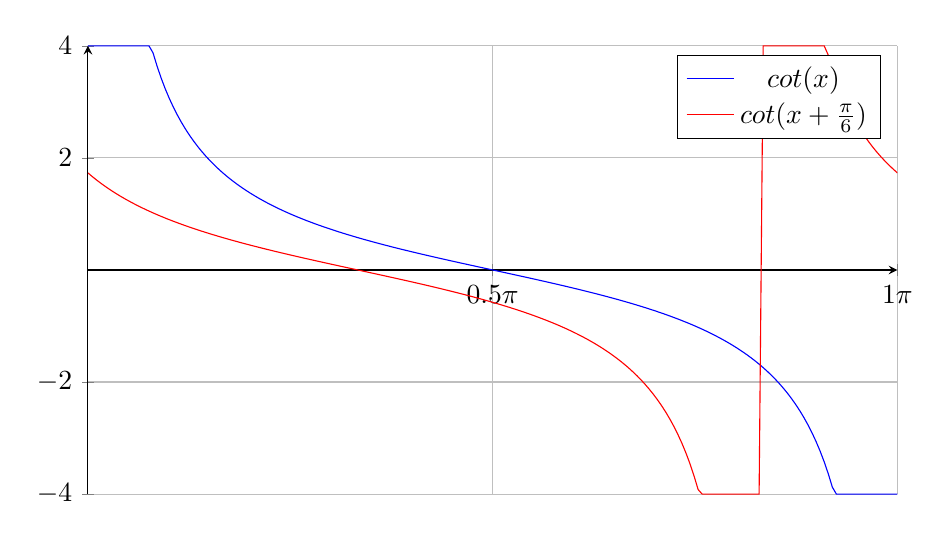
\begin{tikzpicture}
        \begin{axis}
            [
            grid=both,
            axis lines=middle,
            domain=0:pi,
            %restrict x to domain*= -pi:pi,
            restrict y to domain*= -4:4,
            samples=200,
            no marks,
            xticklabels={-2$\pi$,-1.5$\pi$,...$\pi$,2$\pi$},
            xtick={-6.2832,-4.7124,...,6.2832},
            x post scale=1.5
            ]
            \addplot {cot(deg(x))};
            \addlegendentry{$cot(x)$};
            \addplot {(cot(deg(x + (pi / 6))))};
            \addlegendentry{$cot(x + \frac{\pi}{6})$};
        \end{axis}
    \end{tikzpicture}
\end{solution}


\pagebreak


\begin{problem}[25]
    Show that the function $f(x) = \sqrt{2}\sin(x) + \sqrt{2}\cos(x) + 1$ is a sinusoid by rewriting it in the forms $C(x) = A\cos(\omega x + \phi) + B$ and $S(x) = A\sin(\omega x + \phi) + B$ for $\omega > 0$ and $0 \leq \phi < 2\pi$.
\end{problem}

\begin{solution}[Solution]
    This makes absolutely zero sense to me and the book is far too dense for me to understand it. So I'll do what couple steps I can.
    
    \[ \sqrt{2}\sin(x) + \sqrt{2}\cos(x) + 1 =  A\sin(\omega x) \cos(\phi) - \cos(\omega x) \sin(\phi) + B\]
    
    I'm going to assume that $\omega$ here is 1 as is $B$. I THINK $A = \sqrt{2}$ but I'll get to that in a second.
    
    \[ \sqrt{2}\sin(x) + \sqrt{2}\cos(x) + 1 =  A\sin(1 x) \cos(\phi) + \cos(1 x) \sin(\phi) + 1\]
    
    From here based on the book I think I need to use the pythagorean identity? We can assume that $A\cos(\phi) = \sqrt{2}$ same with sine. So. 
    
    \[(\sqrt{2})^2 + (\sqrt{2})^2 = A^2\]
    \[ 4 = A^2\]
    \[ A = 2\]
    
    So at this point I have the following thing going on here.
    
    \[ \sqrt{2}\sin(x) + \sqrt{2}\cos(x) + 1 =  2\sin(1 x) cos(\phi) + 2 \cos(1 x) sin(\phi) + 1 \]
    
    What this means is as good a guess as any. I really do not understand where to go from here or if I'm even following along correctly. Figured I would give it a shot at least though.
\end{solution}
\end{document}

%\addplot {(tan(deg(x - (pi / 3))))};